\section{Autonomous Workflow and Reliability}
\subsection{What the controller actually automates}
The incident orchestrator accepts a typed incident specification, fixed Source Watch audit inputs and resource budgets. In execution mode its code-owned registry can call the existing allowlisted web collector. Seed URLs do not automatically enlarge that registry or its domain allowlist. Newly returned capture manifests can pass through the ingest bridge into a run-local evidence ledger. Optional typed offline inputs can then be processed. Dry-run planning, collection execution, and local analysis are explicit independent options.

The offline runner invokes lineage, retrieval, typed timeline organization, information summaries, supplied conflict inputs, uncertainty scenarios and report checks where compatible inputs exist. It records absent inputs as blocked or not run rather than fabricating them. Retrieval does not invoke the dedicated curated claim-builder's acceptance heuristics. Report generation expects a separately supplied bundle containing findings, evidence records and verification results. Thus a successful controller execution is not evidence that raw sources were transformed autonomously into verified findings. Figure~\ref{fig:workflow} shows the decisive boundary.

\begin{figure}[tbp]
\centering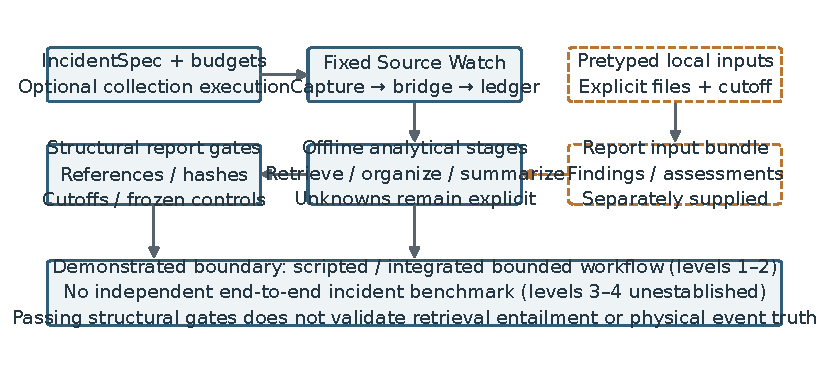
\includegraphics[width=\linewidth]{analysis_workflow.pdf}
\caption{Bounded workflow and automation boundaries. Typed inputs, curated judgments and separately run media analysis enter through explicit interfaces. Structural gates can reject invalid references; they cannot turn a candidate passage into a semantically warranted finding. The end-to-end investigative claim remains unvalidated.}
\label{fig:workflow}
\end{figure}

\subsection{An explicit descriptive autonomy scale}
For this paper, level~0 means manual operation; level~1 scripted processing of supplied inputs; level~2 an integrated automated analytical workflow; level~3 evidence-aware autonomous search and assessment within independently validated tasks; and level~4 independently validated end-to-end analysis on incidents with initially unknown results. This is an author-defined descriptive scale, not a community standard or an ordinal accuracy measure.

Most collectors, local indexing and curated builders operate at level~1. The typed offline runner and limited orchestrator demonstrate level~2 integration. Their semantic inputs and conclusions remain bounded by supplied data and unmeasured inference quality. A separately executed heuristic claim builder does not raise the whole system to level~3; no current result demonstrates level~4. Human or externally validated reference sets are needed during development and evaluation, but this does not imply a human must label every future record in production. Rather, unsupported production tasks must remain unknown or outside the validated operating envelope.

\subsection{Reliability gates and uncertainty}
The evaluation harness checks schema shape, references, time cutoffs, source dependencies, report artifact hashes and frozen synthetic scenarios. It explicitly marks semantic evaluation not evaluated. In particular, 783 passing tests cannot imply 100\% factual accuracy. Structural acceptance provenance such as \code{validated_rule} does not establish that a rule was independently validated. Fixed heuristic confidence values are not calibrated probabilities.

Uncertainty scenarios expose dependence on disputed labels, unknown channel groups, removal/capping assumptions and concentrated observations. Their intervals are scenario bounds conditional on the supplied records, not sampling confidence intervals for population opinion. Incremental dispatch and report differences can identify affected outputs and changed decisions, but do not guarantee that a revised substantive conclusion is true. The engineering priority is transparent failure and inspectability, consistent with reproducible research practices \citep{sandve2013reproducible,wilson2017practices}; semantic reliability remains a separate empirical obligation.
